\documentclass[crop, tikz]{standalone}
\usepackage[utf8]{inputenc}
\usepackage[english, serbianc]{babel}
\usepackage{tikz}
\usetikzlibrary{calc}
\usetikzlibrary{calc, arrows.meta, positioning, backgrounds}
\usetikzlibrary{perspective}

\begin{document}
	\begin{tikzpicture}
		\node[anchor=south west,inner sep=0] (image) at (0, 0) {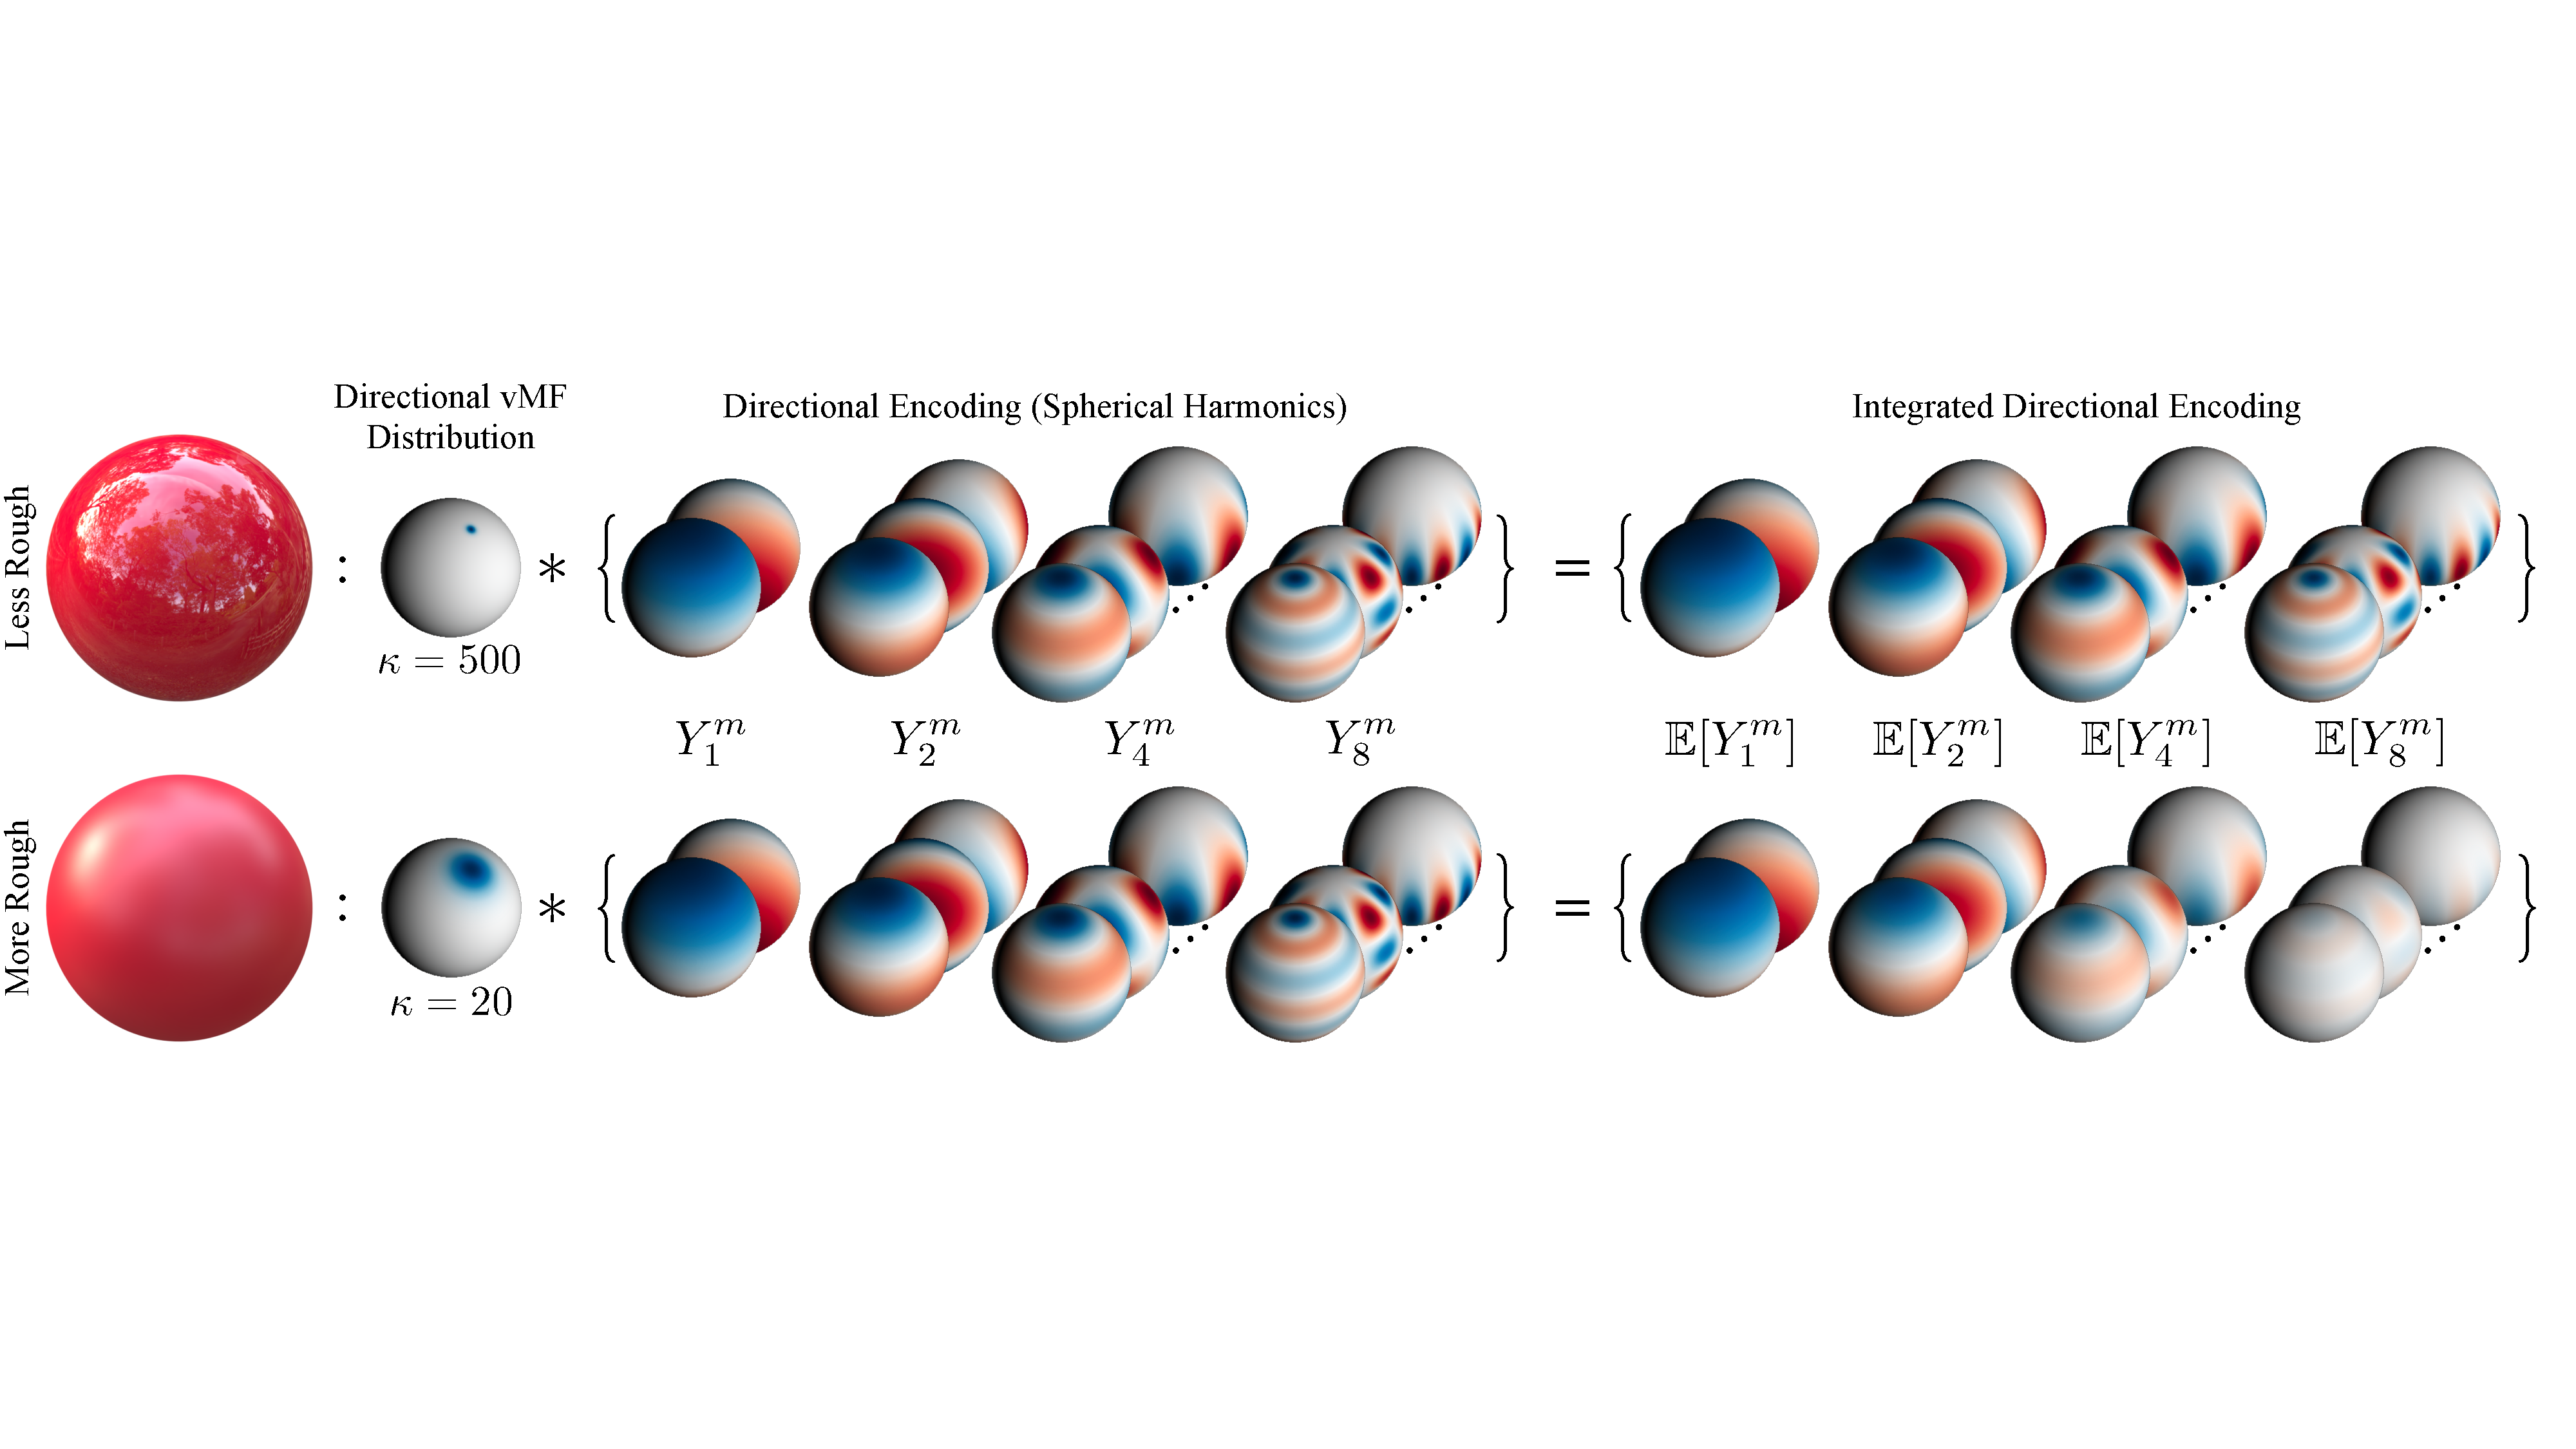
\includegraphics[width=\textwidth]{img/refnerf_ide.pdf}};
		\begin{scope}[x={(image.south east)},y={(image.north west)}]
			\fill[white] (0, 0) rectangle (0.015, 1);
			\fill[white] (0, 0.93) rectangle (1, 1);
			\fill[white] (0.12, 0.88) rectangle (0.24, 1);
			\node[font=\scriptsize] at (0.18, 0.9) {vMF};
			\node[rotate=90,font=\scriptsize] at (0, 0.73) {спекуларно};
			\node[rotate=90,font=\scriptsize] at (0, 0.22) {дифузно};
			\node[font=\scriptsize] at (0.42, 0.95) {сферни хармоници};
			\node[font=\scriptsize] at (0.82, 0.95) {сферна фуријеизација};
		\end{scope}
	\end{tikzpicture}
\end{document}